\documentclass[11pt]{article}

% ---------- packages ----------
\usepackage[margin=1in]{geometry}
\usepackage[utf8]{inputenc}
\usepackage[T1]{fontenc}
\usepackage{amsmath,amssymb}
\usepackage{booktabs}
\usepackage{array}
\usepackage{longtable}
\usepackage{graphicx}
\usepackage{caption}
\usepackage{enumitem}
\usepackage{hyperref}
\usepackage{xcolor}
\usepackage{textcomp}

\hypersetup{
  colorlinks=true, linkcolor=blue, citecolor=blue, urlcolor=blue,
  pdftitle={A Frame-Exact Reinforcement Learning Environment from a Shipped Game Binary, with Procedural Track Generation},
  pdfauthor={Rohan Khandelwal, Vihaan Choudhary},
  pdfsubject={Reinforcement learning environments; simulation fidelity; procedural content generation},
  pdfkeywords={reinforcement learning, simulation fidelity, procedural content generation, out-of-distribution generalisation, racing games, test-time search}
}
\captionsetup{labelfont=bf, labelsep=period}

\newcolumntype{L}[1]{>{\raggedright\arraybackslash}p{#1}}
\newcolumntype{C}[1]{>{\centering\arraybackslash}p{#1}}

\title{\textbf{A Frame-Exact Reinforcement Learning Environment from a Shipped Game Binary, with Procedural Track Generation}}
\author{Rohan Khandelwal \and Vihaan Choudhary}
\date{}

\begin{document}

\maketitle

\begin{abstract}
Reinforcement-learning environments for racing are usually built by reimplementing a game's dynamics, so their fidelity to the game is rarely measured. We build one the other way for PolyTrack, a commercial browser racing game: we host the game's own compiled WebAssembly physics and capture its collision geometry from the shipped client, rather than rebuilding either. The result is frame-exact against two complementary validation oracles (\S3.3): all ten human laps the game recorded for us, on five tracks and up to 61,428 frames long, replay to their recorded finish frame, and the game's own replay verifier, run unmodified, agrees with our agents' banked laps. These two checks are complementary rather than fully independent, since both ultimately execute the same hash-identical physics module (\S3.3). A procedural generator writes track codes the game loads and returns each track's route by construction, so new tracks need no human lap. Policies trained on 48 generated tracks finish all 16 held-out tracks drawn from the same generator, at $97.9 \pm 0.6\%$ of attempts over three seeds, but none of four official, human-designed tracks. A separate, single longer run (1.22M gradient steps) shows no measurable gap between performance on its own training tracks and on held-out tracks from the same generator (92\% against 94\%), which rules out simple memorisation of the 48 training layouts; these are two different experiments and we report them as such. We measure why official tracks fail in observation space: official tracks sit 147--154 times further outside the policy's training support than unseen generated tracks do, with the gap opening as the attempt proceeds rather than at its first frame. The failure is distributional, not a ceiling: trained on an official track, the same agent laps it within 2.0\% of the best human time. Pretraining on generated tracks gives mixed transfer over three seed pairs: later first laps, more progress mid-run, and an equal end. A policy-guided beam search laps one official track in 18.786~s, 23~ms faster than the best human lap available to us, though the winning search was steered by that lap's own racing line and selected from a much larger pool of logged search configurations (\S6.3).
\end{abstract}

\noindent\textbf{Keywords:} reinforcement learning environments $\cdot$ simulation fidelity $\cdot$ procedural content generation $\cdot$ out-of-distribution generalisation $\cdot$ racing games $\cdot$ test-time search

\section{Introduction}

The strongest results in racing reinforcement learning were obtained inside the real game. Sony AI's Gran Turismo Sophy (``GT Sophy'') achieved superhuman wheel-to-wheel racing (Wurman et al., 2022); its time-trial predecessor (Fuchs et al., 2021) and Linesight's world-record Trackmania laps all trained against the game's true dynamics. Research environments without that access reimplement the dynamics instead, and a reimplementation's fidelity to the original is rarely measured. Hosting rather than reimplementing has precedent elsewhere in RL -- Gym Retro hosts emulated console ROMs and Malmo drives the real Minecraft client (\S2) -- but, to our knowledge, not yet for a browser-native, WebAssembly-compiled physics engine with no public API, which is the specific problem this paper solves. We flag this as a claim based on a targeted rather than exhaustive literature search (\S2); we cannot rule out a similar implementation existing elsewhere.

The gap matters because a racing policy optimises a trajectory to the very edge of the dynamics it trained against. If those dynamics differ from the game's, the resulting lap is not a lap of that game. Section~3.4 gives an instance from this work: a collision mesh wrong by $1.8 \times 10^{-4}$ was invisible and drivable at 308~km/h, yet threw a 400~km/h wall-ride off the track thirteen seconds later.

PolyTrack, a browser racing game by Kodub, makes the alternative possible. Its physics ships as a WebAssembly module that steps deterministically at 1~ms per frame. We host that module directly, capture its collision geometry from the running client, and check the result against two complementary oracles the game itself provides (\S3.3). The paper makes five claims and no others, ordered by the strength of their evidence (Table~\ref{tab:claims}):

\begin{table}[h]
\centering
\small
\begin{tabular}{@{}cL{5.2cm}L{5.2cm}c@{}}
\toprule
\textbf{Claim} & \textbf{Statement} & \textbf{Evidence} & \textbf{Strength} \\
\midrule
C1 & A faithful environment can be built from a shipped game binary by hosting its physics and capturing, not reimplementing, its geometry; the result is frame-exact against two complementary validation oracles, which are not fully independent since both execute the same physics module (\S3.3). & 10 of 10 human laps on five tracks reproduce their recorded finish frame; the game's own verifier agrees with every banked lap (\S3.3). & Strong \\
\addlinespace
C2 & A procedural generator writes track codes the game loads and yields each track's route by construction, retiring the human-lap bootstrap. & 31 of 31 shipped tracks re-encode exactly; 24 of 24 generated tracks are drivable (\S4). & Strong \\
\addlinespace
C3 & A policy trained on generated tracks generalises to held-out tracks drawn from the same generator, not to the full distribution of PolyTrack tracks in general. & Three seeds, $97.9 \pm 0.6\%$ of held-out attempts finished (\S6.1). A separate, single longer run shows no measurable train/held-out gap within the generated distribution: 94\% held-out against 92\% training (\S6.1). These are two different experiments. & Strong \\
\addlinespace
C4 & Failure on human-designed tracks is distance in observation space, and the measurement points to where a policy fails. & A control arm and a confound arm (\S6.2); official tracks are learnable when trained on (\S6.4). The localisation is a post-hoc reading and the distance-causes-failure link is not yet tested directly (\S8.1). & Medium \\
\addlinespace
C5 & Policy plus test-time search beats the best human lap on an official track. & 18.786~s against 18.809~s on one track, $n=1$, with the search steered by a human racing line and selected from 186,387 logged search rollouts across the project (\S6.3). & Medium \\
\bottomrule
\end{tabular}
\caption{The paper's five claims, ordered by the strength of their evidence.}
\label{tab:claims}
\end{table}

C1 is the contribution; C2--C5 show that the environment supports real research questions. C5 is the claim most open to attack and the least load-bearing, and we report it with its caveats rather than as a headline.

The measurement behind C4 is not specific to racing. Saying that a policy fails on human-designed levels because they are out of distribution is a claim about the observation space, so we test it there: against the band of observations the policy actually saw, with a control arm of unseen in-distribution tracks and a confound arm that isolates the one asymmetry in how the two track sets are built. The same protocol applies wherever an agent trained on generated tasks is evaluated on tasks the generator did not produce.

Section~2 places the work among racing agents and benchmarks. Section~3 describes the environment and its validation, Section~4 the generator, and Section~5 the agent and search. Section~6 reports results, Section~7 lists what they do not show, and Section~11 revisits the five claims above in light of the results.

\section{Related work}

The strongest racing agents were trained inside real games, and the strongest racing benchmarks are purpose-built simulators; none of either offers a reusable environment whose fidelity to a shipped game has been measured.

\paragraph{Racing RL.} GT Sophy (Wurman et al., 2022) reached superhuman wheel-to-wheel racing in Gran Turismo Sport. Its time-trial predecessor (Fuchs et al., 2021) established the template this work follows most closely: a dense course-progress reward rather than sparse finish time, observations in the car-local frame, and explicit lookahead of upcoming geometry. Vision-based successors (Vasco et al., 2024; Lee et al., 2025) show that pixels are possible but harder, which argues for structured state when the simulator can provide it.

\paragraph{Trackmania.} Linesight (pb4 \& Agade, 2024) is the strongest public agent, using a modified Implicit Quantile Network (IQN) over discrete keyboard inputs with a reference-line reward; in May 2024 it beat ten of twelve world records on the official campaign tracks of Trackmania Nations Forever. TMRL (Bouteiller \& Geze) is the most reusable open framework, using Soft Actor-Critic (SAC) and Randomized Ensembled Double Q-learning (REDQ) over LIDAR-style observations. Both operate the real game, and neither offers a reusable, fidelity-validated environment to third parties, which is the gap this work addresses.

\paragraph{Racing benchmarks.} Macaluso et al. (2024) provide a Trackmania-inspired Unity environment with a Gymnasium interface (Towers et al., 2024), built for offline RL, and comparable Unity-based racing environments with published baselines exist elsewhere in the offline-RL literature. F1TENTH (O'Kelly et al., 2020) is the main scaled-autonomy benchmark, and its survey (Evans et al., 2024) finds that optimisation-and-tracking pipelines achieve the fastest laps, followed by online planning, ahead of end-to-end learning, a result \S6.3 is consistent with. These are purpose-built simulators, built to resemble a racing game or to model a physical scaled vehicle; none claims frame-exact agreement with a shipped commercial title's own physics, because none runs that title's own code.

\paragraph{Hosting the real engine, elsewhere.} Hosting a shipped engine rather than reimplementing it is not a new strategy in general. Gym Retro (Nichol et al., 2018) runs real emulated console ROMs for exactly this reason, and the Malmo platform (Johnson et al., 2016) drives the actual Minecraft client rather than a reimplementation of it. Neither targets a browser-native, WebAssembly-compiled physics engine with no public API and no file-based asset format, which is the specific engineering problem Sections~3.1--3.2 solve. We narrow our claim accordingly: the contribution here is a method for this class of target -- extracting a compiled module with no documented interface and capturing geometry by intercepting a running client's internal messages -- not the general idea of hosting over reimplementing, which is established practice elsewhere. This comparison rests on a targeted literature search rather than a systematic one, and we cannot rule out other instances of this pattern in genres or platforms we did not survey.

\paragraph{Algorithms.} We use Implicit Quantile Networks (IQN; Dabney et al., 2018) with prioritised replay (Schaul et al., 2016) and $n$-step returns, in the multi-collector, single-learner arrangement of Ape-X (Horgan et al., 2018) also used by Linesight and Fuchs et al. (2021).

\paragraph{Generalisation.} Procedural content generation substantially improves generalisation in RL (Justesen et al., 2018). PolyTrack's portable track codes make an effectively unbounded track distribution available, which \S4 exploits.

\paragraph{Learned policy plus test-time search.} Pairing a fast learned policy with test-time search is the pattern behind AlphaZero (Silver et al., 2018) and, recently, superhuman Stratego (Sokota et al., 2025). Section~5.3 applies it to racing.

\section{The environment}

The environment runs PolyTrack's own physics and geometry, and reproduces every human lap the game recorded for us to the millisecond. This section describes how it is built (3.1--3.2), how it is validated (3.3--3.4), what the agent perceives (3.5) and what it costs (3.6). Figure~\ref{fig:environment} summarises the overall architecture.

\begin{figure}[htbp]
    \centering
    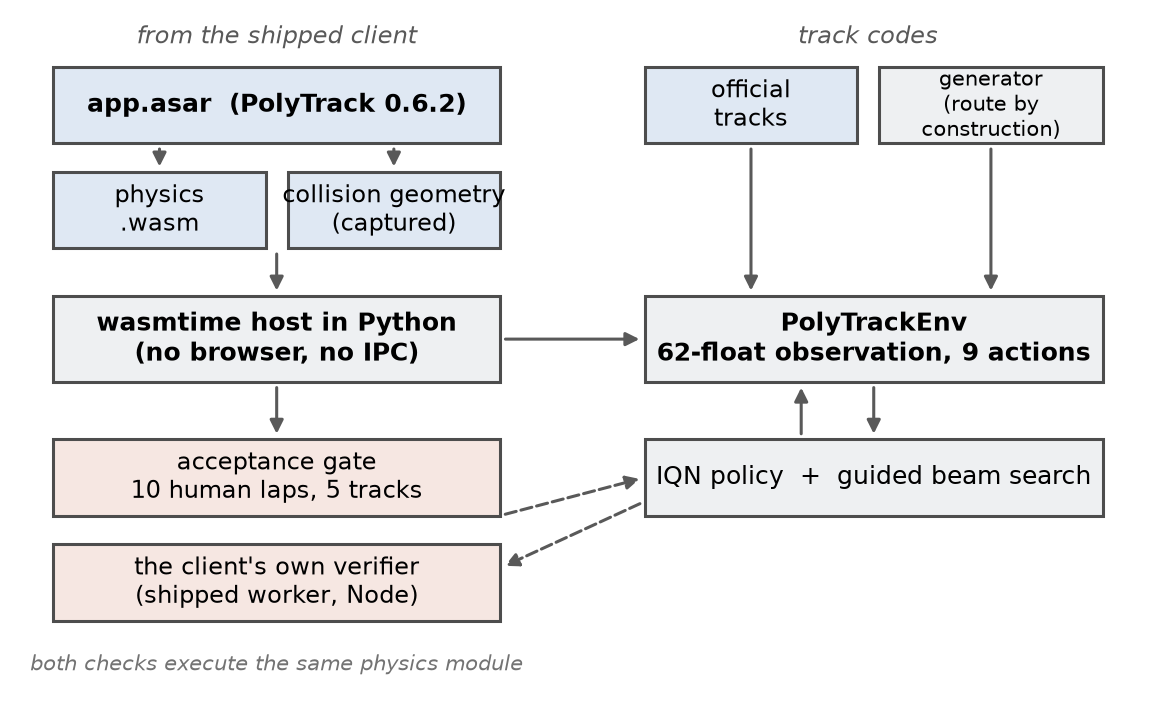
\includegraphics[width=0.85\textwidth]{figures/fig1_architecture.png}
    \caption{The environment. The game's own physics module and its captured collision geometry are hosted in Python; track codes come from the official tracks or the generator. The acceptance gate replays human laps through the hosted physics, and the client's own verifier re-runs the agents' laps.}
    \label{fig:environment}
\end{figure}

\subsection{Hosting the game's own physics}

PolyTrack moved its physics to WebAssembly in version 0.4.0 and rewrote most of it in C++ in 0.6.0. We load the shipped \texttt{polytrack\_physics.wasm} in Python through the \texttt{wasmtime} runtime. The copy used throughout this paper was extracted from client version 0.6.2, the same version in which all ten acceptance-gate laps were recorded and verified (Table~\ref{tab:gate}); we have not tested whether frame-exactness holds against the module shipped in other 0.6.x releases, and treat that as an open reproducibility risk rather than a settled point (\S9.2). All nine of its imports are ordinary Emscripten hooks, and only heap resizing needs a real implementation, so there is no browser, no Node process and no inter-process communication in the loop.

One frame is one millisecond. Three independent details in the shipped client confirm it: the simulation worker drains its time accumulator in 0.001~s steps, \texttt{maxFrames} is 5,999,999 (99:59.999 counted in milliseconds), and the time formatter divides frame counts by 60,000 and 1,000. Community notes for an earlier version state 60~Hz and quote the same \texttt{maxFrames} in one sentence; the two cannot both hold.

A thousand decisions a second is not a usable action space, so an agent holds one of nine discrete actions for a control interval of 50~ms. The nine actions are the cross product of three throttle states (accelerate, brake, neither) and three steering states (left, right, neither). The hot path then makes one seven-argument call into the module per simulated millisecond. We call exports through the raw C API rather than the Python wrapper, which boxes every argument: about $4\,\mu$s against $100\,\mu$s for a seven-argument call. At 1000 calls per simulated second that is roughly 4~ms against 100~ms of wrapper overhead per simulated second -- non-trivial, though smaller than the module's own 650--800~ms per simulated second of compute (\S3.6); together the two costs, not the wrapper alone, motivated avoiding it.

\subsection{Capturing rather than reimplementing geometry}

The one input the client's JavaScript does not describe is the collision geometry, which is compressed inside the game's 3D models. We serve a local copy of the client over loopback, install a hook ahead of its deferred bundles, and intercept the initialisation message it sends to its own simulation worker. That message carries the collision vertices of all 186 part types verbatim.

As a cross-check we also reimplemented the extraction pipeline in three.js, the library the game uses, and matched 185 of 186 parts bit for bit. The one it missed, part 159 (StraightTilted), is the subject of \S3.4. Capture is therefore the primary path, and the reimplementation is kept only for its checksums, which is what localised the failure.

\subsection{Validation against two complementary oracles}

The two checks below answer different questions and fail in different ways, so we use both, but we avoid calling them ``independent'': both ultimately execute the same compiled, hash-identical physics module, so neither can independently confirm that module's own correctness against the original game. What they do establish, and do not, is stated precisely below. This two-check design -- one external and behavioural, the other internal and code-level -- is a standard differential-testing pattern in software verification rather than a novel method in itself; the contribution here is applying it carefully to a compiled game binary with no public API.

\paragraph{The acceptance gate (external, behavioural check).} For each personal best the game stores the input recording and the frame on which the run finished. Replaying the recording through our host must land on that frame exactly, not approximately: a simulator 0.01\% off finishes a 40-second run 4~ms early, more than the margins in \S6.3. The game runs the same check on its own replays, and \texttt{polytrack/verify.py} mirrors that loop. A recording alone cannot serve as an oracle, because it ends when the last key is released rather than when the run ends. This check tests whether our hosted module, driven by real recorded human inputs, reproduces the game's recorded outcome; it cannot by itself prove the module is bug-free in states no recorded lap visited (\S7).

\begin{table}[h]
\centering
\small
\begin{tabular}{@{}lccc@{}}
\toprule
\textbf{Track} & \textbf{Recorded finish (frames)} & \textbf{Reproduced} & \textbf{Recorded}$^{\dagger}$ \\
\midrule
Desert 3  & 21,778 & 21,778 & \\
Summer 1  & 23,805 & 23,805 & \\
Summer 1  & 24,125 & 24,125 & \\
Summer 1  & 24,778 & 24,778 & \\
Summer 5  & 57,037 & 57,037 & \\
Summer 5  & 61,428 & 61,428 & \\
Winter 4  & 19,980 & 19,980 & * \\
Winter 5  & 18,809 & 18,809 & * \\
Winter 5  & 19,025 & 19,025 & \\
Winter 5  & 21,899 & 21,899 & \\
\bottomrule
\end{tabular}
\caption{The acceptance gate, re-run on all ten laps on 22 October 2026: every human lap in \texttt{records.json} lands on its recorded finish frame, a drift of zero frames everywhere. All ten were played by the authors in game version 0.6.2. $^{\dagger}$Unmarked rows were recorded before 21 Oct 2026; rows marked * were recorded on 21 Oct 2026, after the discount-flag fix of \S5.2.}
\label{tab:gate}
\end{table}

\paragraph{The client's own verifier (internal, code-level check).} The gate validates our host's behaviour against recorded human play, but for a lap our own search produced, the target frame is our own claim rather than a pre-existing record. We therefore run the shipped simulation worker unmodified under Node and send it the initialisation and verification messages the game itself sends. It decodes the track with its own decoder and deserialises the recording with its own codec. It agrees with all four Winter 5 laps we put to it (19.025, 18.809, 19.422 and 18.786).

The verifier exercises our track-code encoder, our recording codec and our call sequence against the game's own code. It does not independently confirm the physics itself, because both sides run the same module, hash-identical; a latent bug in that module would pass both checks. The two checks are complementary in a narrower sense than ``independent oracles'' suggests: the gate says our hosted module reproduces the game's recorded outcomes, and the verifier says we drive and encode for that module the way the game's own client does. Confirming the module's fidelity against ground truth the module itself cannot produce -- e.g.\ against an entirely separate reimplementation, or against telemetry the original game does not expose -- remains outside what either check can do, and we list it as a priority in \S8.3.

\subsection{A small geometry error with a large consequence}

The one collision mesh our reimplementation got wrong was off by $1.8 \times 10^{-4}$. It was invisible, and the car drove over it at 308~km/h without incident. Thirteen seconds later it threw a 400~km/h wall-ride clean off the track, on Winter 5 only; the other three tracks we then had oracles for were unaffected.

The size of a geometry error is no guide to the size of its consequences, and no amount of inspection substitutes for an exact replay test. We consider this the strongest single argument for the method of \S3.1--3.3.

\subsection{What the agent perceives}

An environment can be faithful in its dynamics and still mislead in its observations, and ours did. The observation includes rangefinder-style rays after Fuchs et al. (2021), which originally measured distance from the reference line and treated anything beyond a nominal width as a wall. Where a driven lap hugged one side of the road, that reported a wall on open tarmac.

The rays now march through a grid built from the real collision geometry, in which each cell holds a vertical occupancy bitmask. Validation requires a real human lap to be on the ground for its whole length, a test that passes only if the part transform, the rasterisation and the height query are all correct together. It rejected three plausible designs:

\begin{table}[h]
\centering
\begin{tabular}{@{}lc@{}}
\toprule
\textbf{Model} & \textbf{Share of a real lap reported off the ground} \\
\midrule
Keep the $N$ highest surfaces per cell & 33\% \\
Count only upward-facing surfaces & 14\% \\
Symmetric height tolerance & 15\% \\
\bottomrule
\end{tabular}
\caption{Three candidate collision-surface models and the share of a real human lap each incorrectly reports as off the ground; all three were rejected in favour of the full occupancy-grid model described in the text.}
\label{tab:groundmodel}
\end{table}

The second is a finding about the game rather than a bug: the car drives on walls. The human Winter 5 record wall-rides at 400~km/h along pieces whose supporting faces are vertical, so a benchmark that defined drivable surface by surface normal would silently misreport a seventh of that lap. Because a map that called everything solid would also pass, a second test requires the map to tell road from void: 100\% of the lap reads as solid, against 59\% at 10~m to the side and 0.5\% at 80~m. A track's map takes 1.9~s to build, and nine rays cost $109\,\mu$s against the 50~ms control interval.

\subsection{Cost on two machines}

On a hybrid-core Windows laptop\footnote{Exact CPU models and core counts for both machines are recorded in the repository's hardware notes (\S9.1) rather than in the main text, since development used more than one machine of each class over the project. The qualitative distinction that matters for \S10 is big.LITTLE core scheduling on the Windows laptop versus fanless thermal throttling on the MacBook Air.} the module costs 650--800~$\mu$s per simulated millisecond, nearly independent of track size, so the cost is the module's own fixed work. One collector there yields about 11 transitions a second at a 50~ms control interval, and six give 50--80.

On an M5 MacBook Air (16~GB, fanless) six collectors give 190--230 transitions a second and the learner 115--144 gradient steps a second. Under sustained load the fanless machine throttles to 35--100 gradient steps a second, and room cooling restores most of it. Wall-clock budgets on laptops are therefore not stable, which \S10 returns to.

Capturing the whole 24~MB module state costs 13.9~ms, against 14.4~s to replay a 19-second lap from frame zero: a factor of a thousand, and what makes anchored search affordable (\S5.3).

\section{Procedural track generation}

The generator writes track codes the game itself loads and returns each track's route by construction, which removes the human lap every new track otherwise needs before training (C2). The generator itself is a standard self-avoiding-walk level generator (cf. Justesen et al., 2018); the work required was adapting it to PolyTrack's binary track-code format and part-rotation semantics (\S4.1), not the layout algorithm itself.

A track code is a compressed list of placed parts. We implement an encoder as well as a decoder, validated three ways: every shipped track that decodes at all (31 of 31) re-encodes to identical parts, environment and sun direction; the client's own worker loads a track rebuilt from parsed parts, and all three banked laps still verify frame-exactly on it; and unit tests cover the edge cases.

The generator lays out self-avoiding walks on the game's grid, placing a start, straights, right-angle corners, checkpoints and a finish. Because the walk is the route, a generated track carries its own reference line. Before this, a route came only from replaying a lap a human had driven, so no new track could be trained on until somebody drove it.

24 of 24 generated tracks with corners are drivable. A scripted pure-pursuit driver finished 23 of them at its default corner speed of 11~m/s, in 36--47~s and through every checkpoint, and the 24th at 9~m/s. Each had 30 pieces and 4--8 corners. These 24 tracks were generated and checked separately, early in development, purely to validate the generator's geometry; they are not part of either the 48-track training library or the 16-track held-out library used in Section~6, which were generated afterward from disjoint seed ranges (0--47 and 1000--1015 respectively). Those libraries sample length and corner density per track: 48 training tracks from seeds 0--47 (375--1,145~m, 3--19 corners) and 16 held-out tracks from seeds 1000--1015 (374--1,124~m, 3--16 corners). A track's par time is the scripted driver's time halved.

\subsection{Two findings from building it}

\paragraph{Part orientation is not what the start transform implies.} The transform that places the car composes the part's rotation with a half turn about the vertical axis, but parts themselves are placed without it. A straight piece is symmetric under a half turn, so every check built from straight-only tracks passed under the wrong model, including full drives to the finish. Only corners expose it: we built one corner at all four rotations and drove each, and exactly the two the corrected model predicts were drivable.

\paragraph{A check can measure the wrong thing and look like proof.} An adjacency test reported zero broken connections on a track no car could drive. It measured how far each piece's geometry reached toward its neighbour, and a barrier reaches a boundary exactly as well as an opening does. Its replacement keeps only upward-facing surfaces and asks where road actually exists.

\subsection{Its narrowness}

The vocabulary is narrow, and we state that rather than defend it. The generator uses five of the game's 186 part types (a start, a straight, one right-angle corner, a checkpoint and a finish) on flat ground, with no jumps, banking, elevation or walls, and at least one straight between corners by default. Two same-handed corners in succession form a $180^\circ$ hairpin inside 40~m that the scripted driver cannot take.

Generated tracks are drivable, which says the geometry is sound, not that they are interesting to race. Section~6.2 measures what the narrowness costs, and \S6.4 is the evidence that the cost is a limit of the generator rather than of learning.

\section{Agent and search}

The agent is a distributional Q-learner trained from parallel collectors, and the search uses it as an action prior. Every banked result used the configuration below, including a discount the code's own default argues against (\S5.2).

\subsection{Policy}

We use IQN (Dabney et al., 2018) over nine discrete actions (\S3.1), with prioritised replay (Schaul et al., 2016), 5-step returns and a Double-Q bootstrap (van Hasselt et al., 2016). Several collector processes feed one learner, the Ape-X arrangement (Horgan et al., 2018) also used by Linesight and Fuchs et al. (2021).

The observation is a 62-float vector in the car's frame, with speed-scaled lookahead of upcoming geometry after Fuchs et al. (2021) and GT Sophy (Wurman et al., 2022). It holds local velocity and speed, angular velocity, an airborne flag, four wheel-contact flags, lateral offset from the reference line, 20 lookahead points (40 values) and nine rays (\S3.5). These sum to the full 62 dimensions: local velocity (3), speed (1), angular velocity (3), the airborne flag (1), four wheel-contact flags (4), lateral offset (1), lookahead (40) and rays (9). Distributional value estimation suits racing: committing to a corner at speed either works or puts the car into a wall, and the mean of those two futures describes neither.

\begin{table}[h]
\centering
\small
\begin{tabular}{@{}lL{9cm}@{}}
\toprule
\textbf{Component} & \textbf{Setting} \\
\midrule
Network & MLP $62 \rightarrow 256 \rightarrow 256$, a 64-term cosine embedding of the quantile fraction merged multiplicatively, 9 outputs \\
Quantile samples & 8 and 8 in the loss; 32 when acting \\
Optimiser & Adam, learning rate $5 \times 10^{-5}$, gradient clip 10; target network refreshed every 1,000 steps \\
Returns & 5-step, discount $\gamma = 0.99$ (\S5.2) \\
Replay & Prioritised, 200,000 transitions, $\alpha = 0.5$, $\beta$ annealed from 0.4 to 1 over 500,000 learner steps; batch 128 \\
Collectors & Six processes, each with a fixed exploration rate from 0.4 down to $6.6 \times 10^{-4}$ \\
Control & One action held for 50~ms; a failed episode is cut after 3~s with under 5~m of progress, once a 5~s grace has passed \\
\bottomrule
\end{tabular}
\caption{Training configuration of every banked run.}
\label{tab:trainconfig}
\end{table}

\subsection{The discount every banked run used}

Every banked result was trained at $\gamma = 0.99$, a discount the code argues against. The agent's configuration defaults to 0.999, with a comment that 0.99 is a five-second horizon at a 50~ms control interval, too short to value the far side of a track. The training script's own \texttt{-{}-gamma} flag defaulted to 0.99 and always overrode it. We fixed this on 21 October 2026: the flag now defers to the configuration, and the collectors take their $n$-step discount from the agent's configuration, with a test.

The comparison below was run after that fix, with the \texttt{-{}-gamma} flag removed entirely rather than merely overridden, so the two arms differ only in the discount passed to the agent's configuration and not in which code path produced them.

The longer horizon did not help. On Summer 1, trained from scratch with seed 1, budget and everything else held fixed:

\begin{table}[h]
\centering
\begin{tabular}{@{}lcc@{}}
\toprule
 & $\gamma = 0.99$ & $\gamma = 0.999$ \\
\midrule
First lap, gradient steps & 121k & 344k \\
Share of the lap at 300k steps & 65\% & 38\% \\
Greedy laps completed, of 10 & 10 & 0 \\
\bottomrule
\end{tabular}
\caption{Single-seed comparison of discount factors on Summer 1, all other hyperparameters and the training budget held fixed.}
\label{tab:gammacompare}
\end{table}

This is one seed. It licenses the statement that 0.99 did not handicap the banked results and nothing more, so we did not retrain \S6.1.

\subsection{Policy-guided search}

A beam search over action blocks uses the policy as an action prior: only its top-$k$ actions are expanded, which reduces $9^5 = 59{,}049$ futures five blocks ahead to 243 the policy considers drivable. The beam is anchored part-way through a known lap and carries that lap as a guide at every depth, so the result is bounded below by its seed.

Candidates are scored on progress at equal depth, never on shaped reward. Every candidate at a given depth has burned the same number of frames, so ``furthest along the track'' is ``fastest to here'', which needs no coefficients and admits none of the exploits a shaped reward invites. On Winter 5 the ranking adds a speed lookahead and a charge for distance from the reference line, which matters to \S6.3. Whole-state capture (13.9~ms, \S3.6) makes anchoring affordable, and the backend's exact determinism across save and restore makes it sound.

\subsection{A negative result on reward design}

Our first reward charged a per-second time penalty and forfeited part of the un-driven lap on failure. Twelve minutes of training broke it: with the episode over, a failure costs a fixed amount whenever it arrives, while staying alive keeps paying the clock, so the fastest possible failure wins. The agent learned to drive sideways off the start line; the failure histogram moved from 74\% stalled to 88\% off-track while mean return improved and progress fell to zero.

The obvious repair, charging the full time budget on failure, inverts the exploit rather than removing it. Discounting shrinks any large terminal penalty, so stalling before failing beats failing at once, and the agent learns to sit still.

With every reward term non-negative, a terminal state is worth zero and continuing is worth at least zero, so quitting is never strictly better for any policy, any discount, anywhere on the track. Time pressure then comes from a finish bonus scaled by par over elapsed time. We state the design rule plainly: a negative step reward makes ending the episode attractive; a large terminal penalty makes delaying it attractive. The hazard is known in general, but we have not seen it stated in this form for racing, where it is sharp because failure is always one steering input away.

\section{Results}

Policies generalise within the generated distribution (\S6.1) and fail on official tracks for a reason we can measure (\S6.2), yet learn an official track when trained on it (\S6.4); pretraining helps only partly (\S6.5). With search, one official lap beats the best human time we have by 23~ms (\S6.3). Three seeds support the headline result; the long run, the search and the discount comparison are single samples (\S7).

\subsection{Generalisation to unseen tracks}

Three IQN policies were trained from independent seeds for 300,000 gradient steps each (about 3.2~h, six collectors, all nine actions) on the 48 generated training tracks. Each was evaluated with five greedy attempts on each of the 16 held-out tracks, 240 held-out episodes in all. Greedy is not deterministic here, because IQN samples fresh quantile fractions at every forward pass.

\begin{table}[h]
\centering
\begin{tabular}{@{}lcccc@{}}
\toprule
\textbf{Seed} & \textbf{Tracks finished at least once} & \textbf{Mean finish rate} & \textbf{Median best / par} \\
\midrule
1 & 16 / 16 & 99\% & 1.39 \\
2 & 16 / 16 & 98\% & 1.46 \\
3 & 16 / 16 & 98\% & 1.44 \\
\midrule
Across seeds & $100 \pm 0\%$ & $97.9 \pm 0.6\%$ & $1.43 \pm 0.03$ \\
\bottomrule
\end{tabular}
\caption{Held-out performance of three seeds, 240 held-out episodes in total (80 per seed). Spread is half the range, not a standard deviation, because $n=3$ makes a standard deviation similarly unstable; both should be read as indicative rather than precise. Per-seed means are rounded to the nearest percentage point for readability; the aggregate $97.9\pm0.6\%$ is computed from the unrounded per-episode success rates over all 240 episodes (235/240 $\approx$ 97.9\%) and need not equal the mean of the rounded per-seed figures shown.}
\label{tab:heldout}
\end{table}

A fourth policy was trained for 1,220,000 steps over 28.5 hours and measured on the same held-out library and on 16 of its own training tracks:

\begin{table}[h]
\centering
\small
\begin{tabular}{@{}lcccc@{}}
\toprule
 & \textbf{Tracks} & \textbf{Finished at least once} & \textbf{Mean finish rate} & \textbf{Median best / par} \\
\midrule
Held-out & 16 & 16 / 16 & 94\% & 1.35 \\
Training & 16 & 16 / 16 & 92\% & 1.36 \\
Official, zero-shot & 4 & 0 / 4 & 0\% & --- \\
\bottomrule
\end{tabular}
\caption{The long run on held-out, training and official tracks. (``Beat the scripted driver'' is 16/16, 16/16, and --- respectively.) This is a single run, separate from the three-seed result in Table~\ref{tab:heldout}; both held-out and training tracks here are drawn from the same generated distribution.}
\label{tab:longrun}
\end{table}

There is no measurable generalisation gap in this run, within the generated distribution: 94\% held-out against 92\% on tracks it trained on, and 1.35 against 1.36 on time. What that rules out is memorisation of 48 layouts; it does not establish generalisation beyond the generator's narrow vocabulary (\S4.3, \S7). Four times the compute did not buy reliability (94\% against the three-seed result's 97.9\%, Table~\ref{tab:heldout}), and the long run's own curve fell from 93\% at 987,000 steps to 87\% at 1.22~M. We do not have a confirmed explanation for this decline. Plausible contributors include the prioritised-replay $\beta$ schedule completing at 500,000 steps (Table~\ref{tab:trainconfig}), replay staleness as the policy improves faster than old high-priority transitions are replaced, and slow target-network drift; we did not instrument the run to distinguish between them, and flag this as an open question that a repeated, instrumented run should resolve (\S8.2). The long run bought pace instead of reliability: 1.35$\times$ par against 1.43$\times$, and 1.55$\times$ faster than the scripted driver on held-out tracks (median; range 1.37--1.73). Most of the learning is early, with an 82\% finish rate by 257,000 steps and little change after (Figure~\ref{fig:training}).

\begin{figure}[htbp]
    \centering
    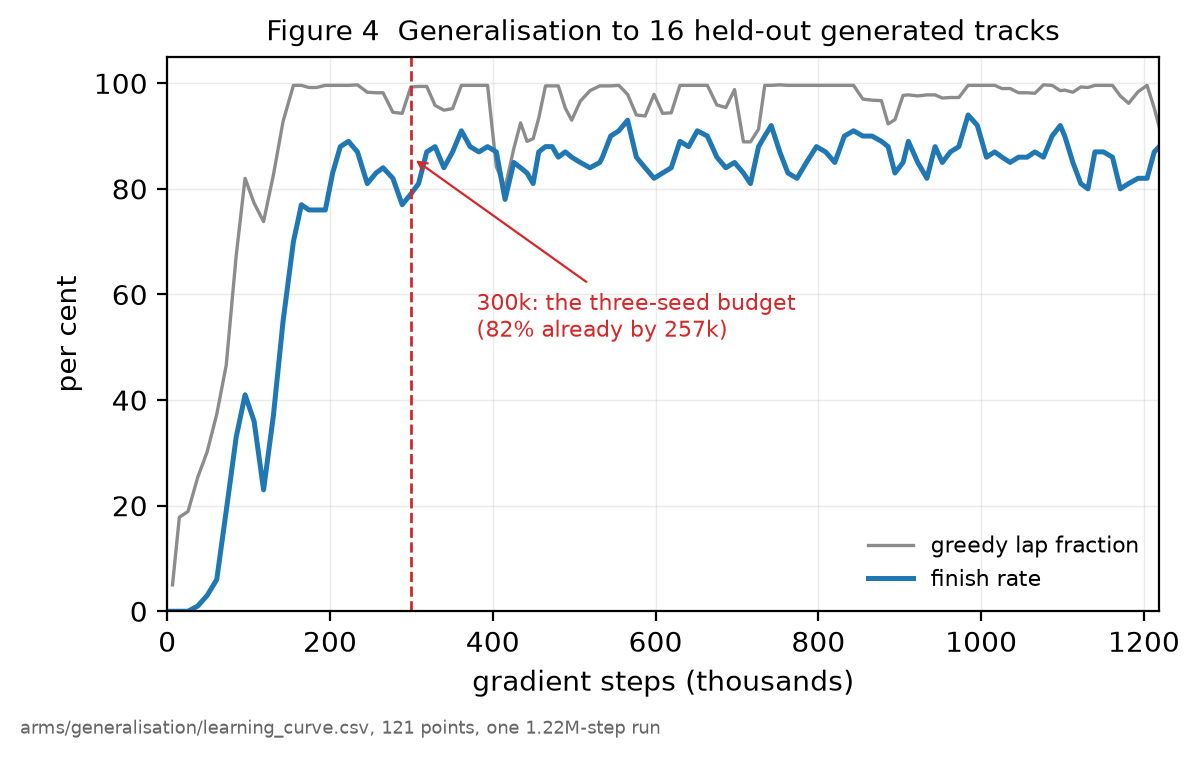
\includegraphics[width=0.85\textwidth]{figures/fig4_generalisation_curve.png}
    \caption{Training on the 48 generated tracks. Blue: share of recent training episodes that finished. Grey: share of the lap reached by the near-greedy collector. The dashed line marks the 300,000-step budget of the three seeds in Table~\ref{tab:heldout}.}
    \label{fig:training}
\end{figure}

The zero-shot row is not a near miss. On the four official tracks the policy reaches 3.1\%, 2.9\%, 23.5\% and 1.5\% of the lap before stalling (Winter 5, Desert 3, Summer 1, Summer 5), three of them within 60~m of the line. Read alone, the row could suggest that official tracks are beyond this agent. Section~6.2 measures what the row does show, distributional distance, and \S6.4 shows it is not a ceiling.

\subsection{The zero-shot gap, measured}

A claim of distributional distance is cheap; telling it apart from a learning failure requires measuring the distance in the space the policy actually consumes, its observation vector. We take the band between the 0.1st and 99.9th percentile of each of the 62 features over the 24,545 frames the 1.22~M-step policy generated while greedily driving its 48 training tracks, and count features outside that band elsewhere. Percentiles rather than extremes, because one outlying frame in twenty-five thousand would otherwise widen a band enough to swallow anything. This is a marginal, per-feature measure: it does not capture novel \emph{combinations} of otherwise in-band feature values, so it can understate distributional distance driven by correlated shifts across features (\S7, \S8.4).

\begin{table}[h]
\centering
\small
\begin{tabular}{@{}L{4.5cm}cc@{}}
\toprule
 & \textbf{Frames with at least one feature outside} & \textbf{Features outside, of 62} \\
\midrule
Control: 16 unseen generated tracks (16 / 16 finished) & 1\% & 0.0--0.1 \\
Test: 4 official tracks (0 / 4 finished) & 57--62\% & 7.0--9.2 \\
\bottomrule
\end{tabular}
\caption{Distance from the training support. Ranges span two passes of the measurement. The control column is rounded to one decimal place for readability; the 147--154$\times$ ratios quoted in the text are computed from the unrounded per-pass counts, which are comfortably above zero in both passes rather than touching it.}
\label{tab:supportdistance}
\end{table}

The control carries the result. An out-of-support count is uninterpretable alone: a band estimated too tightly reports one for every track, including those the policy drives perfectly. Unseen tracks from the training distribution sit inside the band, so the band is not too tight, and the official tracks are 147--154 times further outside it. Greedy action selection is not deterministic under IQN, so the measurement itself carries about $\pm15\%$.

The gap opens during an attempt rather than at its first frame, and not uniformly across tracks. At the first frame the count is one feature of 62 on every official track, which is indistinguishable from noise; an earlier draft of this section read that as the observation being out of support before the car moved, and the per-frame series do not support it. Averaged over the first half of each attempt the count is 7.3 on Winter 5 and 10.0 on Desert 3, against 0.2 on Summer 5 and 0.1 on Summer 1; over the second half it is 14.4, 14.3, 24.5 and 2.8 respectively (Figure~\ref{fig:support}).

So on two of the four tracks the observation is already far outside the training band while the car is still driving, and on the other two it leaves the band as the attempt deteriorates. The distinction matters for what the measurement licenses: where the gap opens late, the distance is \emph{compatible with being a consequence of failing} rather than its cause, since a car against a wall produces velocities and ray readings unlike anything in training. The magnitude is unaffected --- 1.4 to 12.5 features per frame against the control's 0.05 --- and so is the ordering across tracks: Summer 1, which got furthest at 23.5\% of the lap, is the least out of distribution.

\begin{figure}[htbp]
    \centering
    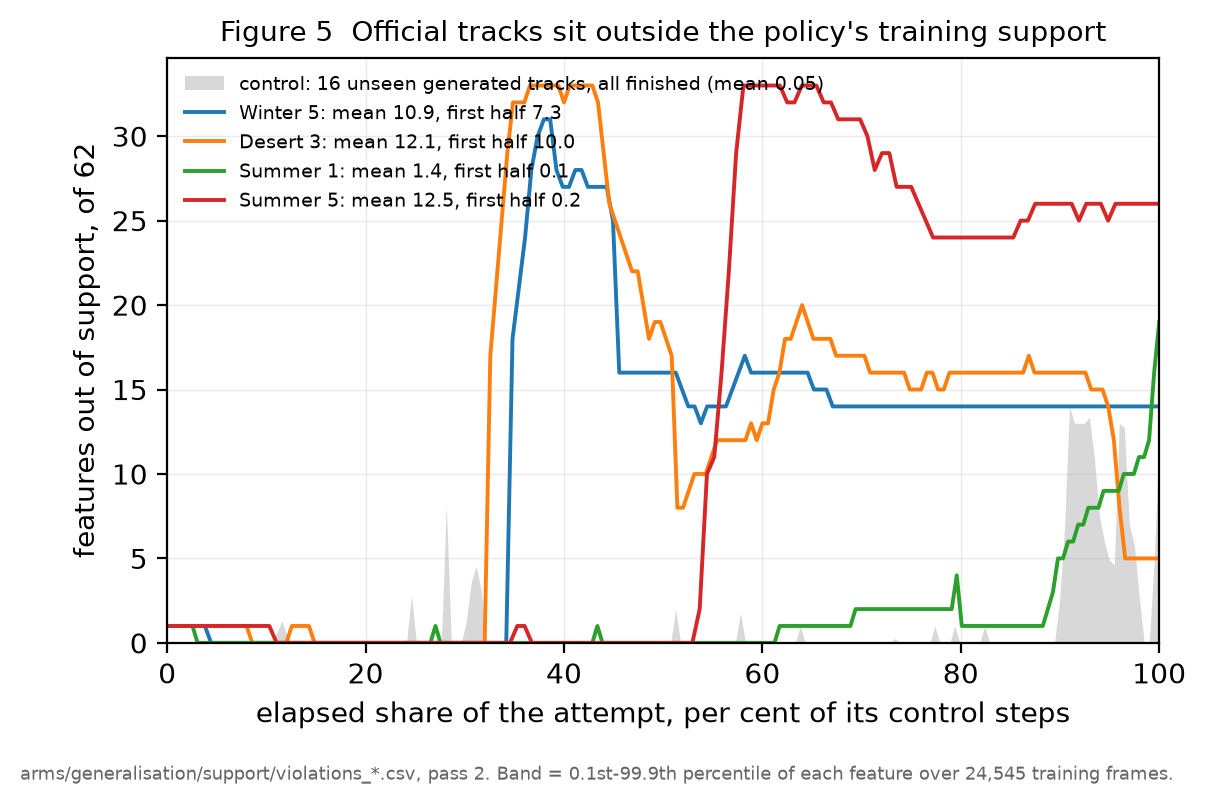
\includegraphics[width=0.85\textwidth]{figures/fig5_out_of_support.png}
    \caption{Features outside the training band over one greedy attempt on each official track, against the elapsed share of that attempt's control steps. The grey band is the control: the same measurement on the 16 held-out generated tracks, every one of which finished. Plotted against elapsed steps rather than distance along the lap, because an attempt that stalls spends many frames at nearly the same arc, which compresses its whole stalled tail against the right-hand edge of a distance axis and makes every track appear to spike late.}
    \label{fig:support}
\end{figure}

\paragraph{Isolating the reference-line confound.} 95\% of the violations fall on the lookahead features, and the lookahead points and lateral offset are measured against the reference line, which the two libraries obtain differently. A generated track's line is its own centreline; an official track's comes from a human lap, and a racing line cuts corners. We therefore changed one variable: 12 training tracks, driven again on the identical road with only the line swapped for one derived from a lap the policy itself drove, built exactly as every official track's line is.

\begin{table}[h]
\centering
\begin{tabular}{@{}lcc@{}}
\toprule
\textbf{Line, on the same 12 roads} & \textbf{Frames with at least one outside} & \textbf{Features outside} \\
\midrule
Centreline (as trained) & 1\% & 0.03 \\
Derived from a driven lap & 20\% & 0.77 \\
Official tracks, for scale & 62\% & 9.2 \\
\bottomrule
\end{tabular}
\caption{The confound arm.}
\label{tab:confound}
\end{table}

Line provenance is a real effect and a small one: 0.77 features per frame against the official tracks' 9.2, at most 8\% of the official-track distance, leaving the road to account for the rest. Two features that no line can confound agree, since nothing about where a line runs makes a car fall or rotate out of the plane: vertical velocity reaches $4.4\times$ beyond the training band on official tracks, and angular velocity about a horizontal axis (roll and pitch) $10\times$. Those are elevation and banking, which a flat grid of right-angle corners cannot express. A two-track pilot of this test reported 1\% and was wrong, because relining changes nothing on some roads and a great deal on others (two of the twelve reach 3.2 and 4.4 features per frame); we report the twelve-track figure.

The distance also points to where policies fail. On Summer 1, policies pretrained on generated tracks lose most of their failed attempts on the valley floor immediately after the 47~m descent (9 of 16), while from-scratch policies lose theirs at the two jumps (11 of 18). Vertical velocity, one of the two features furthest outside the band that no confound explains, is exactly what that descent produces and the generator never does. A distance that also localises a failure is evidence of a mechanism; a distance alone is a correlation. This is a post-hoc reading: the sections below were defined from the reference line's height profile after the runs, not before.

\begin{table}[h]
\centering
\small
\begin{tabular}{@{}L{4cm}ccccc@{}}
\toprule
\textbf{Section of Summer 1} & \textbf{Share of lap} & \textbf{Scratch, $\gamma$ 0.99} & \textbf{Pretrained, $\gamma$ 0.99} & \textbf{Scratch, $\gamma$ 0.999} \\
\midrule
Start plateau, 55~m up & 0--16\% & 4 & 0 & 0 \\
Big descent, 47~m to 1~m & 16--24.5\% & 0 & 0 & 0 \\
Valley floor & 24.5--41\% & 0 & 9 & 0 \\
First jump & 41--53\% & 3 & 0 & 0 \\
Middle plateau & 53--67.5\% & 0 & 1 & 6 \\
Second jump & 67.5--76\% & 8 & 2 & 4 \\
Final plateau & 76--99.5\% & 3 & 4 & 0 \\
\midrule
Finished & --- & 12 & 14 & 0 \\
\bottomrule
\end{tabular}
\caption{Where ten greedy attempts from each final checkpoint end (\S6.5's runs): three seeds per $\gamma$ 0.99 arm, one seed at $\gamma$ 0.999.}
\label{tab:sectionsplit}
\end{table}

\paragraph{What the measurement cannot see.} 12 of the 62 features are bounded and saturated in training (an airborne flag, four wheel-contact flags, and nine ray distances normalised into $[0.083, 1]$ whose full range occurs in training), so they lie outside no band by construction. Every distance reported here is therefore a lower bound. The measurement is also, by design, descriptive rather than causal: it shows the official-track observation is far outside the training band, not that distance itself is what causes the policy to fail (\S7, \S8.1).

\subsection{Search on one official track}

\begin{table}[h]
\centering
\small
\begin{tabular}{@{}L{6cm}L{3.5cm}L{3cm}@{}}
\toprule
\textbf{Winter 5} & \textbf{Time} & \textbf{Verified by} \\
\midrule
Human laps & 19.025~s and 18.809~s & The game's own storage \\
Policy alone, best of 20 greedy laps & 19.422~s & Gate + client verifier \\
Policy + guided beam search & 18.786~s & Gate + client verifier \\
Continuous trajectory optimisation & Did not finish: 1,089~m of 1,747~m & --- \\
\bottomrule
\end{tabular}
\caption{Four approaches to Winter 5.}
\label{tab:winter5}
\end{table}

The search's lap is 23~ms faster than the best human lap available to us (18.809~s, played by an author on 21 October 2026) and 239~ms faster than the earlier human reference (19.025~s). The claim survives at the narrower margin: 18.786~s is the fastest lap on the track we know of, and it is verified by both checks of \S3.3.

The policy was trained on this track with a forward-only action space. That restriction is justified for this track alone: both of the faster human laps hold throttle for 100.0\% of their frames and never brake, including 18.809, whereas every other track in \texttt{records.json} brakes for 8--21\% of the lap. The 19.422 laps were taken at 717,248 gradient steps, from a checkpoint that no longer exists: training continued in the same file, which now holds 801,472 steps, so those twenty greedy laps cannot be redrawn, although the banked lap itself still reproduces. The 860,000 steps that one run reached used a different reference line and produced no banked lap.

\begin{table}[h]
\centering
\begin{tabular}{@{}lcc@{}}
\toprule
\textbf{Search budget} & \textbf{Rollouts} & \textbf{Simulated frames} \\
\midrule
The run that produced 18.786 & 18,309 & 914,944 \\
All logged searches in the project & 186,387 & 9,897,112 \\
Continuous optimisation, all runs & 10,111 & 17,794,080 \\
\bottomrule
\end{tabular}
\caption{Budgets in hardware-independent units.}
\label{tab:budgets}
\end{table}

This single run was selected from 186,387 rollouts logged across all search experiments in the project (Table~\ref{tab:budgets}), so the 23~ms margin reflects the best outcome of substantial search-configuration exploration, not a single blind attempt; we have not corrected for this selection effect, and a more conservative reading would compare the search's typical outcome across configurations rather than its best one.

Three observations matter more than the time.

\paragraph{Search contributes everything.} The policy alone is slower than both human laps, so the whole margin comes from test-time search, consistent with the F1TENTH finding that optimisation-and-tracking beats end-to-end learning on pure lap time (Evans et al., 2024).

\paragraph{The search was steered by a human racing line.} The reference line on this track is the 19.025 human lap, and the ranking term that charges candidates for distance from it found 459~ms in a single run, where seven runs ranking on arc alone had found 14~ms in total. The control sequence is the agent's own, but the route was not discovered independently.

\paragraph{Continuous optimisation failed, informatively.} A separable cross-entropy method over a per-block steering relaxation, seeded from the human lap, spent 17.8~M simulated frames against the 914,944 that produced the finish, and never crossed the line. Winter 5 is chaotically sensitive to millisecond input timing. Projected onto a fixed block grid and replayed, the human lap gets only this far, although at zero timing error it replays exactly:

\begin{table}[h]
\centering
\begin{tabular}{@{}lcccc@{}}
\toprule
\textbf{Grid resolution} & \textbf{50~ms} & \textbf{25~ms} & \textbf{10~ms} & \textbf{5~ms} \\
\midrule
Distance reached, of 1,747~m & 26~m & 349~m & 477~m & 468~m \\
\bottomrule
\end{tabular}
\caption{Input-timing sensitivity on Winter 5.}
\label{tab:timing}
\end{table}

At a two-block spline knot spacing, 97.8\% of the actions are unchanged and the car still reaches only 72~m. That constrains what any trajectory parameterisation can represent on this track.

\subsection{Official tracks are learnable}

A policy trained on Summer 1 laps it in 24.292~s against the best human time of 23.805~s, a difference of 0.487~s, or about 2.05\%, consistent with the 2.0\% figure quoted elsewhere after rounding. Before 21 October no policy with the full action space had completed an official lap; the only official laps were Winter 5's, driven with braking removed (\S6.3). All seven Summer 1 runs of \S5.2 and \S6.5 completed laps within 400,000 gradient steps, with first laps between 121,000 and 344,000 steps. The 24.292~s lap, the fastest training episode across the seven runs, also passes the gate and the client's verifier.

This is what the 0/4 zero-shot row needed beside it. Without it, \S6.1 can be read as ``official tracks are beyond this agent''; with it, the row means what \S6.2 says it means: distributional distance, not a ceiling.

It also changes the label on an earlier experiment. On 20 October we ran the transfer comparison on Summer 1 at a budget of 150,000 steps, a pilot pair at 50,000 and three seeds per arm, and no run in either arm completed a lap. Only one of the seven first laps above falls inside 150,000 steps, and on the easier generated distribution the policy of \S6.1 sat at a 0.67 greedy lap fraction and a 33\% finish rate at 85,000 steps, completing greedy laps only by about 155,000. The 150,000-step experiment was inconclusive at that budget, not evidence of weak transfer. We report it because the budget lesson stands on its own: a censored primary metric cannot compare arms, and a project's own learning curve is the cheapest check on whether a budget can answer the question asked of it.

\subsection{Does the representation transfer?}

We compared three seed pairs on Summer 1 at 400,000 gradient steps and $\gamma = 0.99$. The pretrained arm starts from the generalisation checkpoint's online weights in both networks, with a fresh optimiser and the step counter at zero; the scratch arm starts from random weights. Arms alternated one pair at a time, and the scratch seed-1 run is the $\gamma = 0.99$ run of \S5.2.

\begin{table}[h]
\centering
\small
\begin{tabular}{@{}L{5.5cm}cc@{}}
\toprule
 & \textbf{Scratch} & \textbf{Pretrained} \\
\midrule
First lap, gradient steps (seeds 1 / 2 / 3) & 121k / 234k / 252k & 284k / 246k / 305k \\
First lap, mean & 202k & 279k \\
Share of the lap at 300k steps & 65 / 67 / 65\% & 84 / 93 / 98\% \\
Training episodes finished & 427 / 16 / 71 & 166 / 165 / 157 \\
Greedy laps of 10 & 10 / 0 / 2 & 5 / 8 / 1 \\
Best lap & 24.652 / 28.010 / 25.092~s & 26.084 / 24.292 / 24.833~s \\
\bottomrule
\end{tabular}
\caption{Transfer on Summer 1, three seed pairs.}
\label{tab:transfer}
\end{table}

\begin{itemize}[leftmargin=*]
\item The primary metric goes against transfer. The pretrained arm reached its first lap later in all three pairs.
\item Mid-run progress goes the other way in all three pairs, and the pretrained runs' finished-episode counts are far more consistent across seeds (157--166 against 16--427).
\item The end is a draw: 14 of 30 greedy laps for the pretrained arm against 12 of 30.
\end{itemize}

Three pairs pointing the same way is not significance: a two-sided sign test gives $p = 0.25$, so we report direction and spread rather than a significance claim. ``First lap'' also counts any collector, including the one exploring at a rate of 0.4, so it is noisy by construction; the greedy rows are the cleaner measure of what a policy can do. Figure~\ref{fig:transfercurve} shows the share of the lap reached over training for all six runs.

\begin{figure}[htbp]
    \centering
    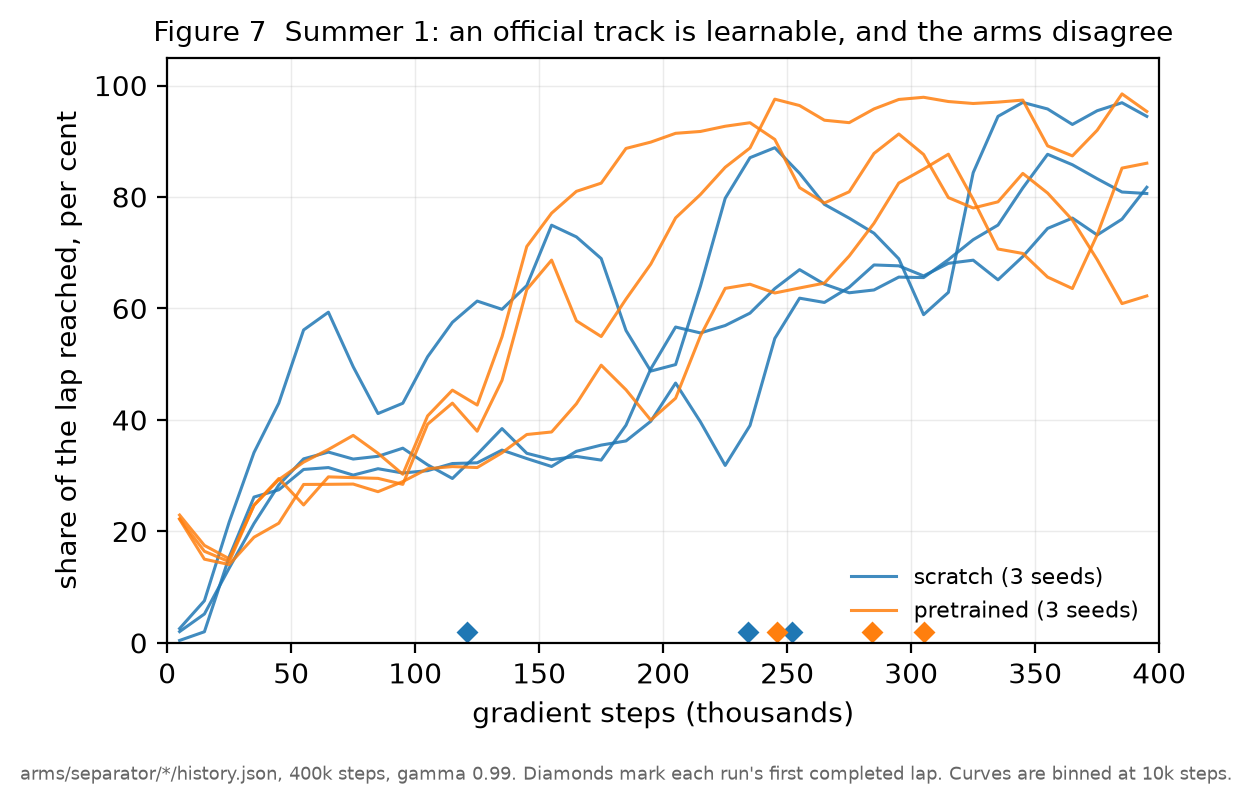
\includegraphics[width=0.85\textwidth]{figures/fig7_summer1_progress.png}
    \caption{Share of Summer 1 reached by the near-greedy collector, averaged over 10,000-step bins, for three seeds per arm at $\gamma = 0.99$. Diamonds mark each run's first completed lap by any collector.}
    \label{fig:transfercurve}
\end{figure}

One reading fits all of it, and we label it as a reading: what transfers is general driving on the parts of a track the generator resembles, and what does not transfer is the part that decides whether a lap completes. The per-section failure split of \S6.2 is consistent with this reading; it is not a test of it.

\section{What this does not show}

The results above are easy to over-read, so we state their limits directly.

\begin{itemize}[leftmargin=*]
\item \textbf{Three seeds, one configuration.} \S6.1 repeats the training run three times, which gives a spread on the headline figure. It does not vary anything else (one architecture, one reward, one set of hyperparameters), so nothing here is an ablation.
\item \textbf{The single-track search results are $n=1$}, and selected from a much larger pool of logged search attempts (\S6.3); it was not repeated under a fixed, pre-registered configuration.
\item \textbf{The discount comparison is one seed.} \S5.2 licenses only the statement that $\gamma = 0.99$ did not handicap the banked results.
\item \textbf{The transfer result is mixed, not null, and it is three seeds.} The primary metric and mid-run progress point in opposite directions, and neither is significant at $n=3$.
\item \textbf{The support measurement is descriptive, not causal, and marginal, not joint.} \S6.2 establishes that the official-track observation lies far outside the per-feature training band and that reference-line provenance does not explain it. It does not show that this distance causes the failure, and it can understate distance driven by correlated shifts across features rather than any single one (\S8.4). The experiment that would settle causality is a wider generator, where the measured distance should fall and performance should follow (\S8.1).
\item \textbf{The per-section failure localisation is post-hoc.} The sections of Summer 1 were read off the reference line's height profile after the runs.
\item 12 of the 62 observation features cannot register a violation, being bounded and saturated in training, so every distance in \S6.2 is a lower bound.
\item \textbf{No learned baseline.} The scripted driver is a floor, not a competitor. Nothing here is measured against Linesight, TMRL, GT Sophy, or a standard algorithm such as PPO or DQN on a common task.
\item \textbf{Par is a convention, not a standard.} On generated tracks it is the scripted driver's time halved, so best/par compares runs within this paper and means nothing outside it.
\item \textbf{The generated distribution is narrow:} five part types on flat ground. \S6.1's zero-shot row measures what that costs, and \S6.2 quantifies it. Generalisation claims in this paper (C3) should be read as generalisation within that narrow distribution, not to PolyTrack tracks in general.
\item The approaches compared on Winter 5 differ along several axes at once and are not a controlled comparison; two share an author, and the third was informed by the second's findings.
\item \textbf{The policy alone does not beat a human on Winter 5.} It is 397~ms slower than the 19.025 lap and 613~ms slower than the 18.809 lap; only policy plus search is faster. On Summer 1, trained on that track, it laps within 2.0\% of the best human time. That is a different statement from the Winter 5 one and should not be conflated with it.
\item \textbf{The environment is validated on five tracks}, against two checks that share the same underlying physics module (\S3.3). Ten runs is a strong gate but a small corpus, and neither check independently confirms the module's fidelity to the original game in states no recorded lap visited.
\end{itemize}

\section{Experiments still required}

The transfer experiment has run and the budget question is settled. One remaining experiment could change what the paper claims, a wider generator (\S8.1); the rest would make the existing claims harder to attack without changing them.

\subsection{Widen the generated distribution}

The generator uses five of 186 part types on flat ground, while the official tracks need jumps, banking, elevation and wall-rides. Each addition is a fresh geometry problem of the kind \S4.1 describes, and elevation in particular turns the self-avoiding walk from a two-dimensional problem into a three-dimensional one.

\S6.2 makes this both targeted and falsifiable. It names the features furthest outside the training band that no confound explains (vertical velocity at $4.4\times$ and angular velocity about a horizontal axis at $10\times$), so elevation and banking come first, and the failure localisation names the Summer 1 valley floor as the first place to look. It also supplies an intermediate measurement: adding a part family should reduce the measured distance on the official tracks, which can be read off before any policy is trained to convergence. If the distance falls and zero-shot performance does not follow, the mechanism claimed in \S6.2 is wrong, and that is the outcome worth being able to detect.

\subsection{Seeds and variance}

\S6.1 has three training seeds, \S6.2 two passes and \S6.5 three seed pairs. The long 1.22~M-step run, every figure in \S6.3, the input-timing results and the discount comparison of \S5.2 remain single samples. What is still wanted is three to five seeds on each configuration, including the search and the discount, and a repeated, instrumented version of the 1.22~M-step run to test the hypotheses in \S6.1 for its late-training decline.

\subsection{Baselines and a stronger validation oracle}

At minimum, one standard algorithm besides IQN, such as PPO or DQN, on the generated tracks and one official track. A comparison against Linesight's method on a common track would be stronger still. The scripted pure-pursuit driver (\S4) remains the floor.

On the validation side, the gate and the client verifier (\S3.3) both execute the same physics module and so cannot independently confirm that module's correctness against the original game in states no recorded lap visited. A genuinely independent check -- for example, telemetry captured directly from the running browser client on inputs never recorded as a personal best, compared frame-by-frame against our hosted module on the same inputs -- would close this gap and is a priority for future work.

\subsection{Ablations}

The observation's lookahead horizon, the action-space restriction, the search's ranking terms, the control interval and the discount.

\subsection{A joint, not marginal, distribution-shift metric}

The percentile-band measurement of \S6.2 is per-feature and marginal; it is a useful first diagnostic but can miss distributional shift that only shows up in combinations of features. A density-ratio estimate, a Mahalanobis-style distance in a whitened feature space, or a classifier trained to distinguish generated from official-track observations would supplement it and should be checked for agreement with the current measurement before either is treated as authoritative.

\subsection{Compute}

Compute is the binding constraint. At 50--80 transitions a second on the Windows laptop, or 190--230 on the M5, tens of millions of transitions take days to weeks of wall-clock time. The workload is CPU-bound and parallel, so it scales nearly linearly with cores; a GPU does not help, since the network is a small MLP.

\section{Reproducibility, licensing and ethics}

Everything we wrote is released; the game's physics module and the geometry derived from it are not ours to release, and that remains the paper's open problem (\S9.2).

\subsection{What is released}

\begin{quote}
\small
\textbf{Repository:} \url{https://github.com/Rohan5054/PolyTrack} \\
\textbf{Release tag used for this paper:} \texttt{paper-v2} \\
\textbf{Physics module hash (SHA-256):} \texttt{d4ef02676973d41afc34b23b5248f695} \texttt{0b35dc4cc7e3047e3a9c6bd88e4c180e} \\
\textbf{Geometry capture hash (SHA-256):} \texttt{6fb32e3b719811dc2204bcf437df4074} \texttt{11769e42e7f455f49d9eda2eaae8eaee} \\
\textbf{Game version required:} PolyTrack 0.6.2 (\S3.1) \\
\textbf{Minimum reproduction command:} \texttt{POLYTRACK\_TRACKS=<tracks> python scripts/run\_gate.py records.json}, expected to reproduce Table~\ref{tab:gate} with zero frame drift on all ten laps. \texttt{scripts/substrate\_hashes.py -{}-json} prints the two hashes above from a local copy, and \texttt{scripts/make\_figures.py} regenerates every figure in this paper from committed data alone.
\end{quote}

The environment, agent, search, generator and scripted driver, with 168 passing tests, and every reported lap as an input recording that replays through the gate. The test suites import the \texttt{polytrack} package, so they need it installed or \texttt{PYTHONPATH=.} set. \texttt{scripts/verify\_baselines.py} re-verifies every lap time in \S6.3 and hashes the inputs they were produced against.

The \S6.2 measurement ships as \texttt{scripts/measure\_support.py} (the band, the control arm and the test) and \texttt{scripts/measure\_line\_confound.py} (the reference-line arm), with both passes' raw logs, the percentile band itself and the group summaries under \texttt{arms/generalisation/support/}. The band is a reusable artifact: re-analysis against a saved band takes minutes, where re-deriving it costs 48 training laps.

The policy itself is released, at \texttt{arms/generalisation/agent.pt} (2.6~MB): the 1.22~M-step checkpoint behind Table~\ref{tab:longrun} and all of \S6.2, with the 48 laps it drove on its training tracks beside it. A checkpoint is 28.5 hours of compute on one machine, so without it the measurement would be described rather than reproducible. It contains 20 weight tensors, optimiser state, hyperparameters and a step count, and no part of the game's content, the same test the released input recordings meet. Both measurement scripts default to these files, so \S6.2 reproduces from a clone plus the two files \S9.2 explains we cannot ship. The separator and transfer runs of \S5.2 and \S6.5 are committed as per-run histories, logs and summaries under \texttt{arms/separator/}.

Two caveats apply to reproducing \S6 exactly. Greedy evaluation is not deterministic under IQN, so finish rates and support distances reproduce to within a few per cent rather than exactly, which is why \S6.2 quotes two passes. And the track libraries embed the game's content, so they are rebuildable from a seed with the released scripts but are not themselves distributable.

\subsection{What cannot currently be released, and why it matters}

The environment depends on the game's compiled physics module and on collision geometry derived from it, and neither is ours to redistribute. A benchmark nobody else can run is not a benchmark, so we state this as an unresolved limitation rather than a detail.

The game's author has confirmed that using the physics module directly is acceptable under the game's terms, and asked that the tooling not permit cheating and not submit runs to the leaderboard. The released code meets both conditions by construction: the replay viewer serves the client on a throwaway local origin and blocks requests to the game's servers at two levels. Redistribution has not been granted and is not addressed by the terms, so reproduction currently requires a copy of the game and an extraction step, a weaker story than a benchmark venue expects. Permission would turn a described environment into one others can run.

PolyTrack is also a live, periodically updated browser game, not a frozen research artifact: a future patch could change the physics module, its WebAssembly export signature, or the geometry formats \S3.2 depends on, which would break frame-exactness silently rather than loudly. Pinning the exact module and asset hashes used in this paper (\S9.1) makes such a break detectable after the fact, but we have no mechanism to guarantee reproducibility of the results in this paper against a version of the game released after it.

\subsection{Ethics and attribution}

All tool-assisted runs are kept off the game's human leaderboard, following the convention Linesight states for Trackmania, and no part of this work interacts with the game's online services. PolyTrack is by Kodub; the official game is available at \url{crazygames.com/game/polytrack}. This work is unofficial and non-commercial, and is not affiliated with or endorsed by Kodub.

\section{An engineering note}

Throughput measured on laptops can be wrong by a large factor in ways that do not look like a throughput problem, and we hit two of them.

\paragraph{Background quality of service on Windows.} On hybrid-core Windows machines, a process the operating system classifies as background work (anything launched detached) is confined to the efficiency cores at their lowest clock. On our machine this cost 52.6~s against 3.6~s on a fixed single-threaded benchmark. On the training loop it moved the achieved ratio of gradient steps to transitions from 0.11 to 0.46, and throughput from 38 to 75 transitions a second. The symptom is deceptive: total CPU reads low, clocks read normal and nothing is thermally limited, which reads as a lock rather than a throttle. The tell is that everything slows by the same factor at once. Every long-running entry point now opts out through the documented power-throttling API, which spawned workers inherit.

\paragraph{Thermal throttling on a fanless laptop.} On the M5 MacBook Air the learner ran at 115--144 gradient steps a second, and under sustained load it throttled to 35--100; room cooling restored most of it.

Both effects change how many transitions and gradient steps an hour buys, and the first also changes the replay ratio the learner achieves. Published throughput figures from laptop experiments may be affected silently, which is why \S6 states budgets in gradient steps and simulated frames rather than hours.

\section{Conclusion}

We set out to build a reinforcement-learning environment that is faithful to a shipped commercial game rather than a reimplementation of it, and to show that such an environment supports real research questions. Table~\ref{tab:claims} summarised five claims; here we revisit them in light of the results.

C1 is supported at the strength we can currently claim: ten of ten human laps reproduce their recorded finish frame exactly, and the game's own verifier agrees with every banked lap we produced. These are two complementary checks rather than fully independent oracles, since both execute the same physics module (\S3.3), and neither can independently confirm that module's fidelity to the original game in states no recorded lap visited (\S8.3). This is the paper's central contribution, and it generalises only as far as the five tracks and ten laps we have validated against, and the single game version tested (\S7, \S3.1). C2 is supported in the same sense: the generator's tracks are drivable by construction and need no human lap, though the vocabulary of part types it draws on remains narrow (\S4.2, \S8.1). C3, read as the two separate experiments it actually is (\S6.1), shows strong within-distribution generalisation on one metric (97.9$\pm$0.6\% of held-out attempts finished, three seeds) and no measurable train/held-out gap on another (94\% against 92\%, a single longer run), both confined to the generator's own narrow distribution rather than PolyTrack tracks in general; neither experiment alone supports both halves of the claim as originally stated, and we have revised the abstract and claims table accordingly. C4's localisation of the generalisation failure to observation-space distance is supported by a control arm and a confound arm, but remains correlational and based on a marginal, per-feature distance measure, rather than causal or joint, until the generator is widened (\S8.1) and the prediction made there is tested. C5 stands at $n=1$, with a 23~ms margin obtained after extensive search-configuration exploration and with the winning route steered by a human racing line; we regard it as suggestive rather than established.

Read together, the results support hosting a shipped game's own physics as a viable, falsifiable way to build a racing RL environment, and they identify where the resulting environment's generated-track distribution still falls short of official human-designed content. The most consequential open question is whether widening the generator (\S8.1) closes that gap, which would convert C4 from a correlation into a tested causal claim; the most consequential open engineering question is whether an independent, non-shared oracle can be constructed to validate the physics module itself (\S8.3).

\begin{thebibliography}{99}

\bibitem[Bouteiller \& Geze]{bouteiller} Bouteiller, Y., \& Geze, E. TMRL: a reinforcement-learning framework for TrackMania [software, MIT licence]. \url{https://github.com/trackmania-rl/tmrl} (version and release date not specified by the authors; accessed 2026).

\bibitem[Dabney et al., 2018]{dabney2018} Dabney, W., Ostrovski, G., Silver, D., \& Munos, R. (2018). Implicit quantile networks for distributional reinforcement learning. \textit{Proceedings of the 35th International Conference on Machine Learning}, PMLR 80, 1096--1105. arXiv:1806.06923.

\bibitem[Evans et al., 2024]{evans2024} Evans, B.~D., Trumpp, R., Caccamo, M., Jahncke, F., Betz, J., Jordaan, H.~W., \& Engelbrecht, H.~A. (2024). Unifying F1TENTH autonomous racing: Survey, methods and benchmarks. arXiv:2402.18558.

\bibitem[Fuchs et al., 2021]{fuchs2021} Fuchs, F., Song, Y., Kaufmann, E., Scaramuzza, D., \& D\"urr, P. (2021). Super-human performance in Gran Turismo Sport using deep reinforcement learning. \textit{IEEE Robotics and Automation Letters}, 6(3), 4257--4264. \url{https://doi.org/10.1109/LRA.2021.3064284}

\bibitem[Horgan et al., 2018]{horgan2018} Horgan, D., Quan, J., Budden, D., Barth-Maron, G., Hessel, M., van Hasselt, H., \& Silver, D. (2018). Distributed prioritized experience replay. \textit{International Conference on Learning Representations (ICLR)}. arXiv:1803.00933.

\bibitem[Johnson et al., 2016]{johnson2016} Johnson, M., Hofmann, K., Hutton, T., \& Bignell, D. (2016). The Malmo platform for artificial intelligence experimentation. \textit{Proceedings of the 25th International Joint Conference on Artificial Intelligence (IJCAI)}, 4246--4247.

\bibitem[Justesen et al., 2018]{justesen2018} Justesen, N., Rodriguez Torrado, R., Bontrager, P., Khalifa, A., Togelius, J., \& Risi, S. (2018). Illuminating generalization in deep reinforcement learning through procedural level generation. arXiv:1806.10729.

\bibitem[Kodub]{kodub} Kodub. PolyTrack [video game], version 0.6.2, as played and extracted for this paper (October 2026). \url{https://www.kodub.com}

\bibitem[Lee et al., 2025]{lee2025} Lee, H., Seno, T., Tai, J.~J., Subramanian, K., Kawamoto, K., Stone, P., \& Wurman, P.~R. (2025). A champion-level vision-based reinforcement learning agent for competitive racing in Gran Turismo 7. \textit{IEEE Robotics and Automation Letters}. \url{https://doi.org/10.1109/LRA.2025.3560873} (arXiv:2504.09021)

\bibitem[Macaluso et al., 2024]{macaluso2024} Macaluso, G., Sestini, A., \& Bagdanov, A.~D. (2024). A benchmark environment for offline reinforcement learning in racing games. \textit{IEEE Conference on Games}. arXiv:2407.09415.

\bibitem[Nichol et al., 2018]{nichol2018} Nichol, A., Pfau, V., Hesse, C., Klimov, O., \& Schulman, J. (2018). Gotta learn fast: A new benchmark for generalization in RL. arXiv:1804.03720.

\bibitem[O'Kelly et al., 2020]{okelly2020} O'Kelly, M., Zheng, H., Karthik, D., \& Mangharam, R. (2020). F1TENTH: An open-source evaluation environment for continuous control and reinforcement learning. \textit{Proceedings of the NeurIPS 2019 Competition and Demonstration Track}, PMLR 123, 77--89.

\bibitem[pb4 \& Agade, 2024]{linesight2024} pb4 \& Agade. (2024). Linesight: a Trackmania AI trained with reinforcement learning [software]. \url{https://github.com/Linesight-RL/linesight}

\bibitem[Schaul et al., 2016]{schaul2016} Schaul, T., Quan, J., Antonoglou, I., \& Silver, D. (2016). Prioritized experience replay. \textit{International Conference on Learning Representations (ICLR)}. arXiv:1511.05952.

\bibitem[Silver et al., 2018]{silver2018} Silver, D., Hubert, T., Schrittwieser, J., et al. (2018). A general reinforcement learning algorithm that masters chess, shogi, and Go through self-play. \textit{Science}, 362(6419), 1140--1144. \url{https://doi.org/10.1126/science.aar6404}

\bibitem[Sokota et al., 2025]{sokota2025} Sokota, S., Vinitsky, E., Hu, H., Fan, Z., Kolter, J.~Z., \& Farina, G. (2025). Scalable decision making for games of imperfect information. arXiv:2511.07312.

\bibitem[Towers et al., 2024]{towers2024} Towers, M., Kwiatkowski, A., Terry, J., Balis, J.~U., De Cola, G., Deleu, T., Goul\~ao, M., Kallinteris, A., Krimmel, M., KG, A., Perez-Vicente, R., Pierr\'e, A., Schulhoff, S., Tai, J.~J., Tan, H., \& Younis, O.~G. (2024). Gymnasium: A standard interface for reinforcement learning environments. arXiv:2407.17032.

\bibitem[van Hasselt et al., 2016]{vanhasselt2016} van Hasselt, H., Guez, A., \& Silver, D. (2016). Deep reinforcement learning with double Q-learning. \textit{Proceedings of the AAAI Conference on Artificial Intelligence}, 30(1). \url{https://doi.org/10.1609/aaai.v30i1.10295}

\bibitem[Vasco et al., 2024]{vasco2024} Vasco, M., Seno, T., Kawamoto, K., Subramanian, K., Wurman, P.~R., \& Stone, P. (2024). A super-human vision-based reinforcement learning agent for autonomous racing in Gran Turismo. arXiv:2406.12563.

\bibitem[Wurman et al., 2022]{wurman2022} Wurman, P.~R., Barrett, S., Kawamoto, K., et al. (2022). Outracing champion Gran Turismo drivers with deep reinforcement learning. \textit{Nature}, 602(7896), 223--228. \url{https://doi.org/10.1038/s41586-021-04357-7}

\end{thebibliography}

\end{document}